\subsection{TargetScan: post-transcriptional repression burden of antigen 3'UTRs}
\label{sec:targetscan}
A tumor antigen's safety margin depends on whether normal-tissue expression
is post-transcriptionally buffered: a 3'UTR dense in conserved miRNA sites
can keep surface protein low even where RNA is detected, while an
unrepressed 3'UTR means RNA presence translates directly to surface
exposure. We audited TargetScan~8.0 default predictions (broadly conserved
miRNA families; 13,037 human genes) for all 205 study genes; a gene
absent from the table has no conserved predicted sites and is recorded as
zero burden.

\paragraph{Calibration gate.} Pre-registered gates PASSED after two recorded
first-pass miscalibrations: (G1) table depth 13,037 human genes (first-pass
threshold 15,000 failed at 13,037; the default table is narrower than the
all-predictions build); (G2) all 205 genes resolved; (G3) the HMGA2
sentinel carries conserved let-7 (GAGGUAG) sites (observed 7 sites),
after two rejected control choices recorded in the audit JSON: essential
housekeeping genes (POLR2A/PCNA carry zero conserved sites, consistent with
short-UTR biology) and KRAS--let-7 (KRAS let-7 sites are not
vertebrate-conserved, and TargetScan is conservation-based).

\paragraph{Burden gated versus background.} Genes carrying at least one
conserved site: 59/99 gated versus 47/98 background (Fisher
odds ratio 1.60, $p=0.117$). Median conserved-site count 1 versus
0 (Mann--Whitney $p=0.466$), median targeting-family breadth 1
versus 0 ($p=0.43$), and median minimum cumulative weighted context++
score -0.092 versus 0 ($p=0.407$). No axis of post-transcriptional repression distinguishes gated antigens from background: miRNA regulation is not a confound of the panel design, and antigen safety margins must be read from RNA/protein abundance directly. Notably, four of seven AND-gate antigens (CA9, CLDN6, MSLN, PSCA) carry ZERO conserved miRNA sites, so their expression is post-transcriptionally unbuffered - RNA presence at these loci translates directly to surface exposure, reinforcing the abundance-based safety windows and marking CLDN18/SLC39A6 (which carry sites) as the only buffered antigens of the set.

\paragraph{AND-gate antigens.} CA9: 0 conserved sites from 0 families; CA12: 13 conserved sites from 13 families; CLDN18: 6 conserved sites from 5 families; CLDN6: 0 conserved sites from 0 families; MSLN: 0 conserved sites from 0 families; PSCA: 0 conserved sites from 0 families; SLC39A6: 4 conserved sites from 4 families.

\begin{figure}[t]
\centering
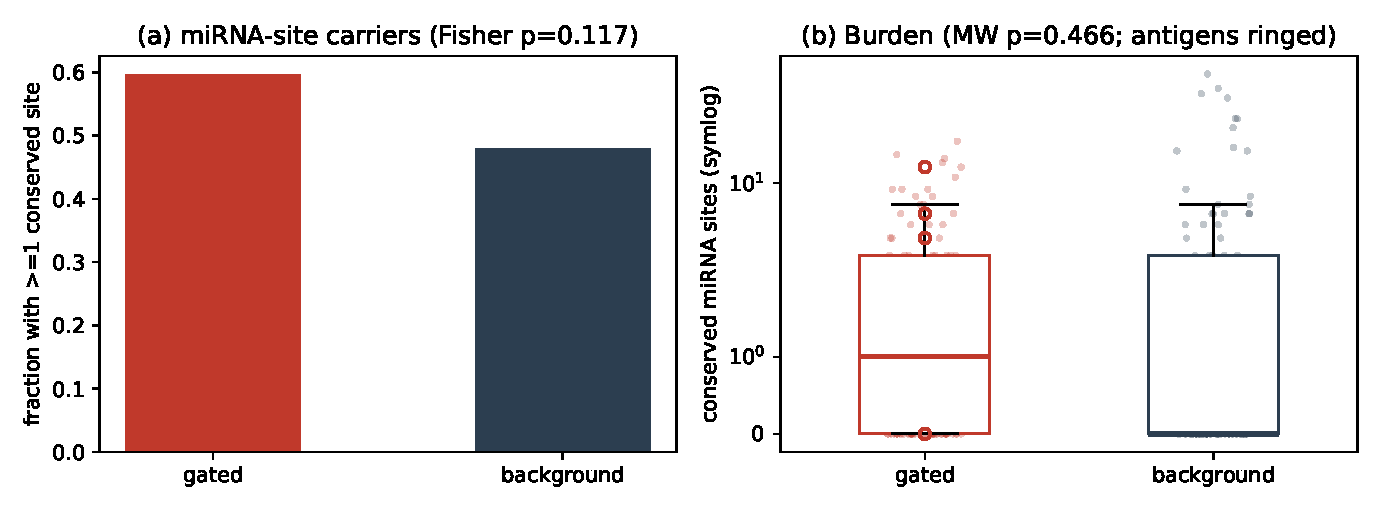
\includegraphics[width=\linewidth]{targetscan_fig.pdf}
\caption{TargetScan miRNA regulatory-burden audit. (a) Fraction of genes
carrying at least one conserved miRNA site. (b) Conserved-site burden per
gene (symlog axis), with the seven AND-gate antigens ringed.}
\label{fig:targetscan}
\end{figure}
